\documentclass[tikz,border=10pt]{standalone}
\usepackage[utf8]{inputenc}
\usepackage[T1]{fontenc}
\usepackage{tikz}
\usetikzlibrary{shapes.geometric}

\begin{document}
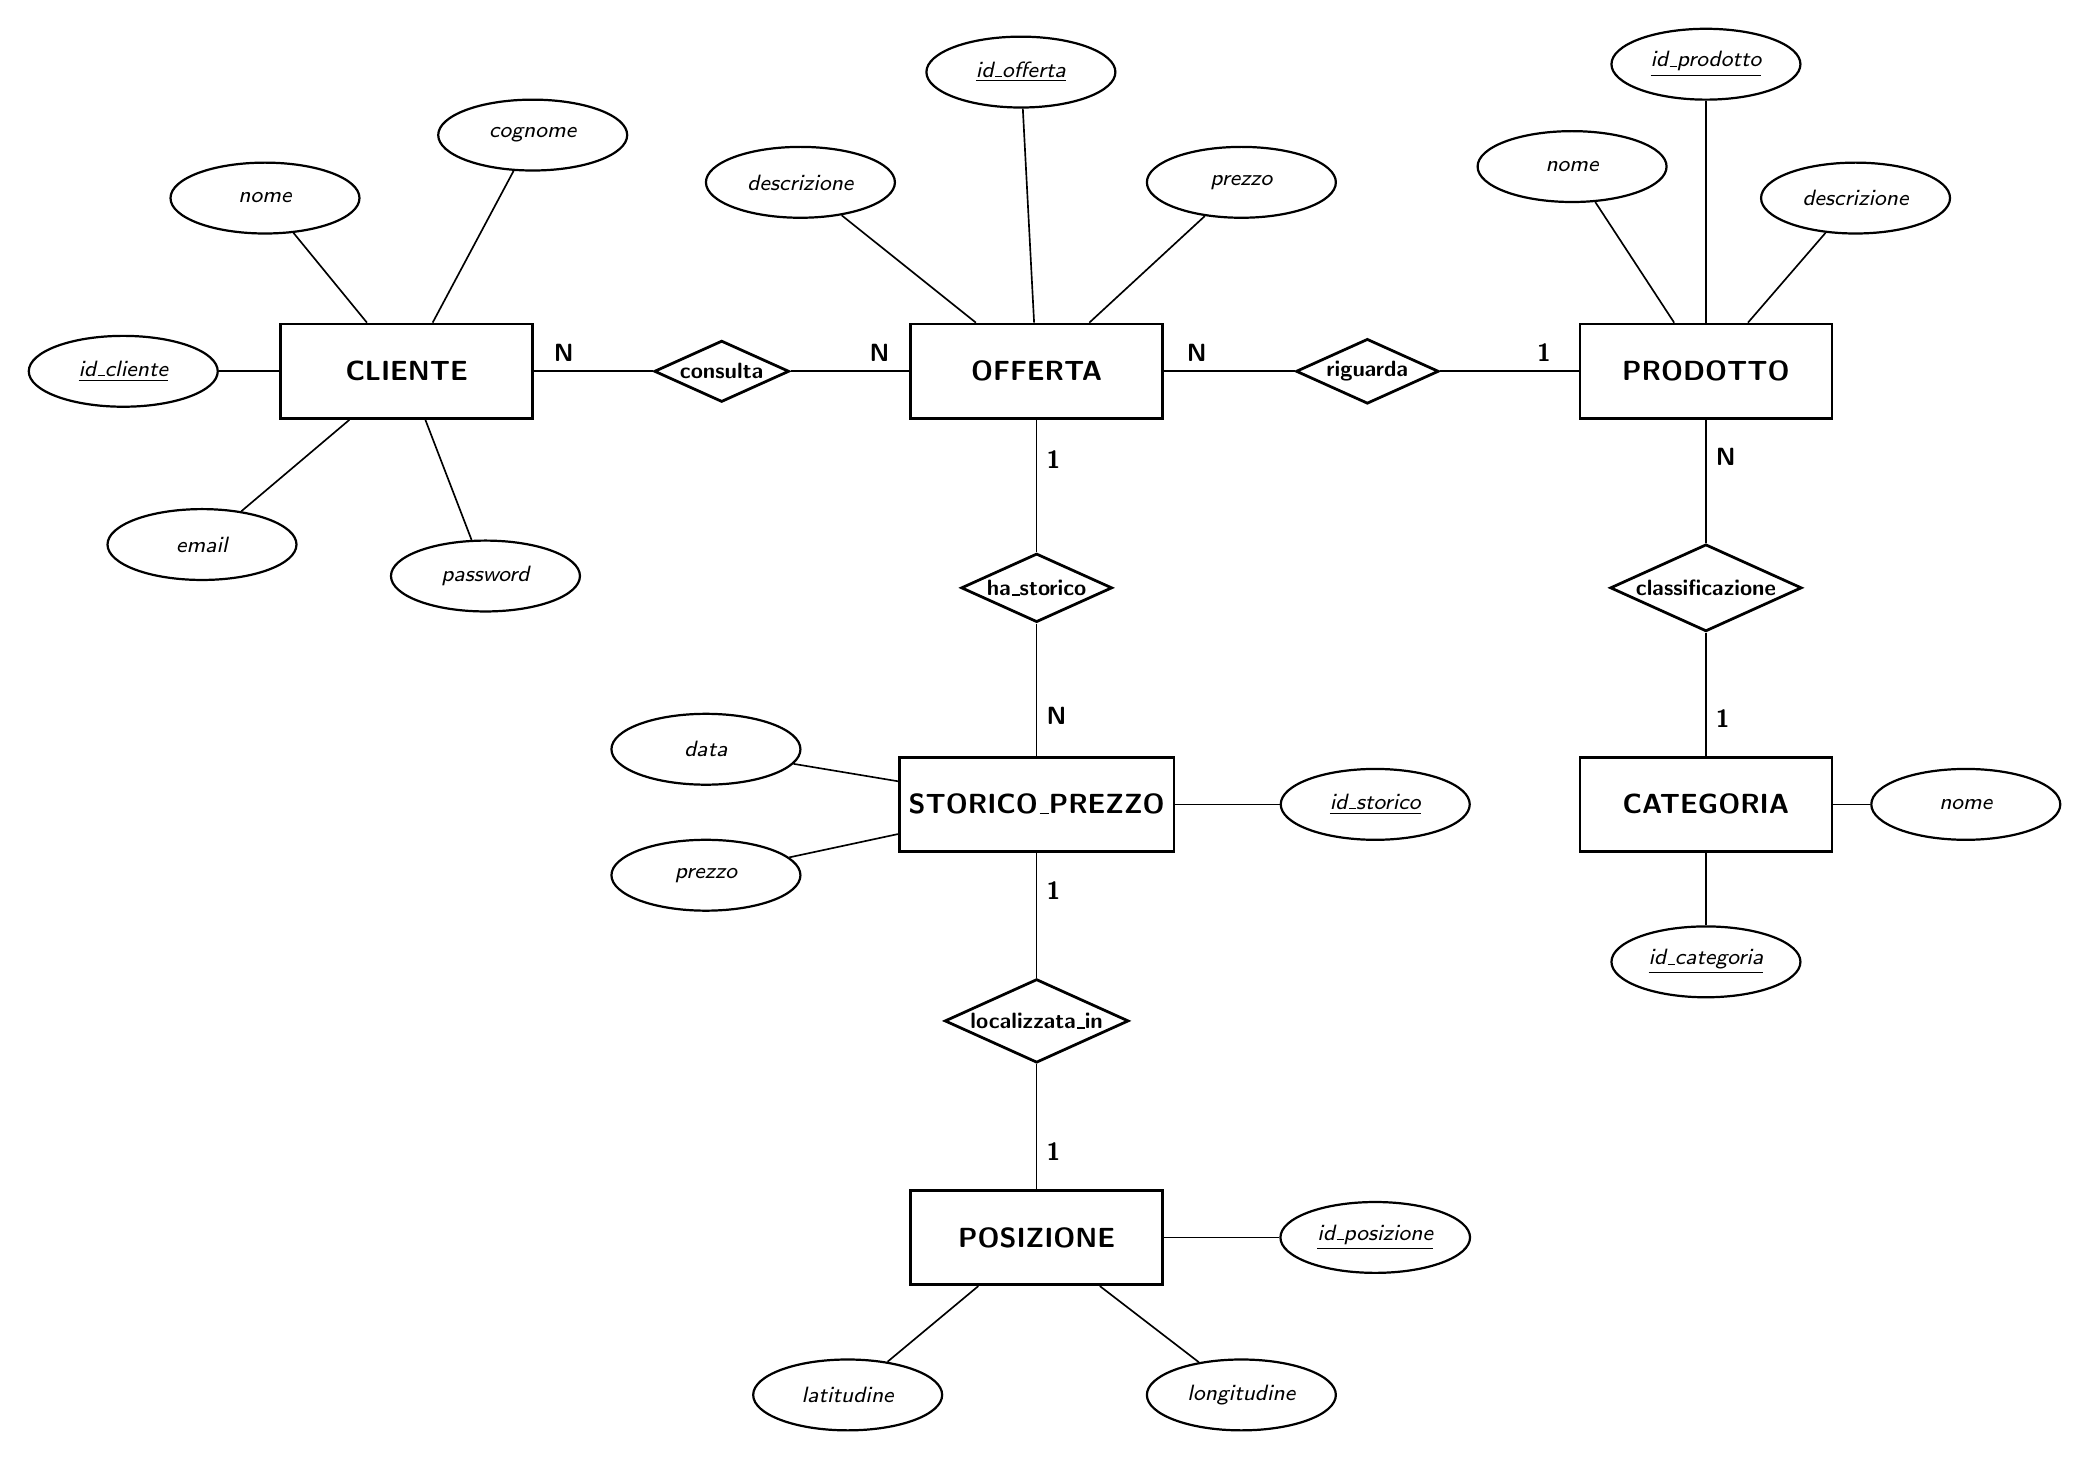
\begin{tikzpicture}[
  font=\sffamily\small,
  line/.style={draw=black, line width=0.6pt},
  entita/.style={rectangle, draw=black, fill=white, line width=1pt,
                 minimum width=3.2cm, minimum height=1.2cm, font=\sffamily\bfseries},
  relazione/.style={diamond, aspect=2.2, draw=black, fill=white,
                    line width=1pt, inner sep=1pt, font=\sffamily\bfseries\footnotesize},
  attributo/.style={ellipse, draw=black, fill=white, line width=0.8pt,
                    minimum width=2.4cm, minimum height=0.9cm, font=\sffamily\itshape\footnotesize},
  card/.style={black, font=\sffamily\bfseries\small}
]

% ---------- ENTITÀ ----------
\node[entita] (cliente)   at (0,0)       {CLIENTE};
\node[entita] (offerta)   at (8,0)       {OFFERTA};
\node[entita] (prodotto)  at (16.5,0)    {PRODOTTO};
\node[entita] (storico)   at (8,-5.5)    {STORICO\_PREZZO};
\node[entita] (categoria) at (16.5,-5.5) {CATEGORIA};
\node[entita] (posizione) at (8,-11)     {POSIZIONE};

% ---------- RELAZIONI ----------
\node[relazione] (consulta)  at (4,0)        {consulta};
\node[relazione] (riguarda)  at (12.2,0)     {riguarda};
\node[relazione] (hastorico) at (8,-2.75)    {ha\_storico};
\node[relazione] (classif)   at (16.5,-2.75) {classificazione};
\node[relazione] (localizz)  at (8,-8.25)    {localizzata\_in};

% ---------- COLLEGAMENTI + CARDINALITÀ ----------
\draw[line] (cliente) -- (consulta)  node[card, pos=0.25, above] {N};
\draw[line] (consulta) -- (offerta)  node[card, pos=0.75, above] {N};

\draw[line] (offerta) -- (riguarda)  node[card, pos=0.25, above] {N};
\draw[line] (riguarda) -- (prodotto) node[card, pos=0.75, above] {1};

\draw[line] (offerta) -- (hastorico) node[card, pos=0.3, right] {1};
\draw[line] (hastorico) -- (storico) node[card, pos=0.7, right] {N};

\draw[line] (prodotto) -- (classif)  node[card, pos=0.3, right] {N};
\draw[line] (classif) -- (categoria) node[card, pos=0.7, right] {1};

\draw[line] (storico) -- (localizz)  node[card, pos=0.3, right] {1};
\draw[line] (localizz) -- (posizione) node[card, pos=0.7, right] {1};

% ---------- ATTRIBUTI (chiavi primarie sottolineate) ----------
% CLIENTE
\node[attributo] (c-id)       at (-3.6,0.0)  {\underline{id\_cliente}};
\node[attributo] (c-nome)     at (-1.8,2.2)  {nome};
\node[attributo] (c-cognome)  at (1.6,3.0)   {cognome};
\node[attributo] (c-email)    at (-2.6,-2.2) {email};
\node[attributo] (c-password) at (1.0,-2.6)  {password};
\draw[line] (cliente) -- (c-id);
\draw[line] (cliente) -- (c-nome);
\draw[line] (cliente) -- (c-cognome);
\draw[line] (cliente) -- (c-email);
\draw[line] (cliente) -- (c-password);

% OFFERTA
\node[attributo] (o-id)     at (7.8,3.8)  {\underline{id\_offerta}};
\node[attributo] (o-descr)  at (5.0,2.4)  {descrizione};
\node[attributo] (o-prezzo) at (10.6,2.4) {prezzo};
\draw[line] (offerta) -- (o-id);
\draw[line] (offerta) -- (o-descr);
\draw[line] (offerta) -- (o-prezzo);

% PRODOTTO
\node[attributo] (p-id)    at (16.5,3.9) {\underline{id\_prodotto}};
\node[attributo] (p-nome)  at (14.8,2.6) {nome};
\node[attributo] (p-descr) at (18.4,2.2) {descrizione};
\draw[line] (prodotto) -- (p-id);
\draw[line] (prodotto) -- (p-nome);
\draw[line] (prodotto) -- (p-descr);

% STORICO_PREZZO
\node[attributo] (s-id)     at (12.3,-5.5) {\underline{id\_storico}};
\node[attributo] (s-data)   at (3.8,-4.8)  {data};
\node[attributo] (s-prezzo) at (3.8,-6.4)  {prezzo};
\draw[line] (storico) -- (s-id);
\draw[line] (storico) -- (s-data);
\draw[line] (storico) -- (s-prezzo);

% CATEGORIA
\node[attributo] (cat-id)   at (16.5,-7.5) {\underline{id\_categoria}};
\node[attributo] (cat-nome) at (19.8,-5.5) {nome};
\draw[line] (categoria) -- (cat-id);
\draw[line] (categoria) -- (cat-nome);

% POSIZIONE
\node[attributo] (pos-id)  at (12.3,-11)   {\underline{id\_posizione}};
\node[attributo] (pos-lat) at (5.6,-13.0)  {latitudine};
\node[attributo] (pos-lon) at (10.6,-13.0) {longitudine};
\draw[line] (posizione) -- (pos-id);
\draw[line] (posizione) -- (pos-lat);
\draw[line] (posizione) -- (pos-lon);



\end{tikzpicture}
\end{document}